\documentclass[journal,12pt,onecolumn]{IEEEtran}

\usepackage{enumitem}
\usepackage{amsmath}
\usepackage{amssymb}
\usepackage{gensymb}
\usepackage{graphicx}
\usepackage{txfonts}
\usepackage{pythonhighlight}

\let\vec\mathbf

\providecommand{\brak}[1]{\ensuremath{\left(#1\right)}}

\newcommand{\myvec}[1]{\ensuremath{\begin{pmatrix}#1\end{pmatrix}}}

\title{Binary Classification \\using Logistic Regression}
\author{Ankit Saha \\ \normalsize AI21BTECH11004 \\ \vspace*{20pt} \normalsize  29 March 2022 \\ \vspace*{20pt} \Large  Report}


\begin{document}

	\maketitle
	
	\section{Problem Statement}
	We are given a red wine data set. This is a classification problem. The goal is to find a model that can classify wine as of:
	\begin{enumerate}
		\item high quality ($1$) or
		\item low quality ($0$)
	\end{enumerate}
			
	\section{Exploratory Data Analysis}
	We first count the number of samples that are labelled as `good quality' and `bad quality' in the entire data set.
	\begin{python}
	good_count = np.sum(df['quality'])
	bad_count = total_count - good_count \end{python}
	where \pyth{total_count} is the total number of samples present in the data set.
	
	This works because the values in the \pyth{'quality'} column are $1$ for 'good quality' and $0$ for 'bad quality'. Thus, only the good quality samples contribute to the sum.
	
	\vspace*{20pt}
	We then use the \pyth{pairplot} function from the \pyth{seaborn} module to plot pairwise relations between a set of 4 variables at a time. We also set the keyword argument \pyth{hue} to \pyth{'quality'} so that we can visualize the contrast between good and bad samples for these comparisons.
	\begin{python}
	ls1 = list(df)[:4] # ['volatile acidity', 'citric acid', 'residual sugar', 'chlorides']
	ls1.append('quality')
	sc1 = sns.pairplot(df.loc[:, ls1], hue='quality')
	plt.savefig('figs/fig-1.png')
	plt.show() \end{python}
	
	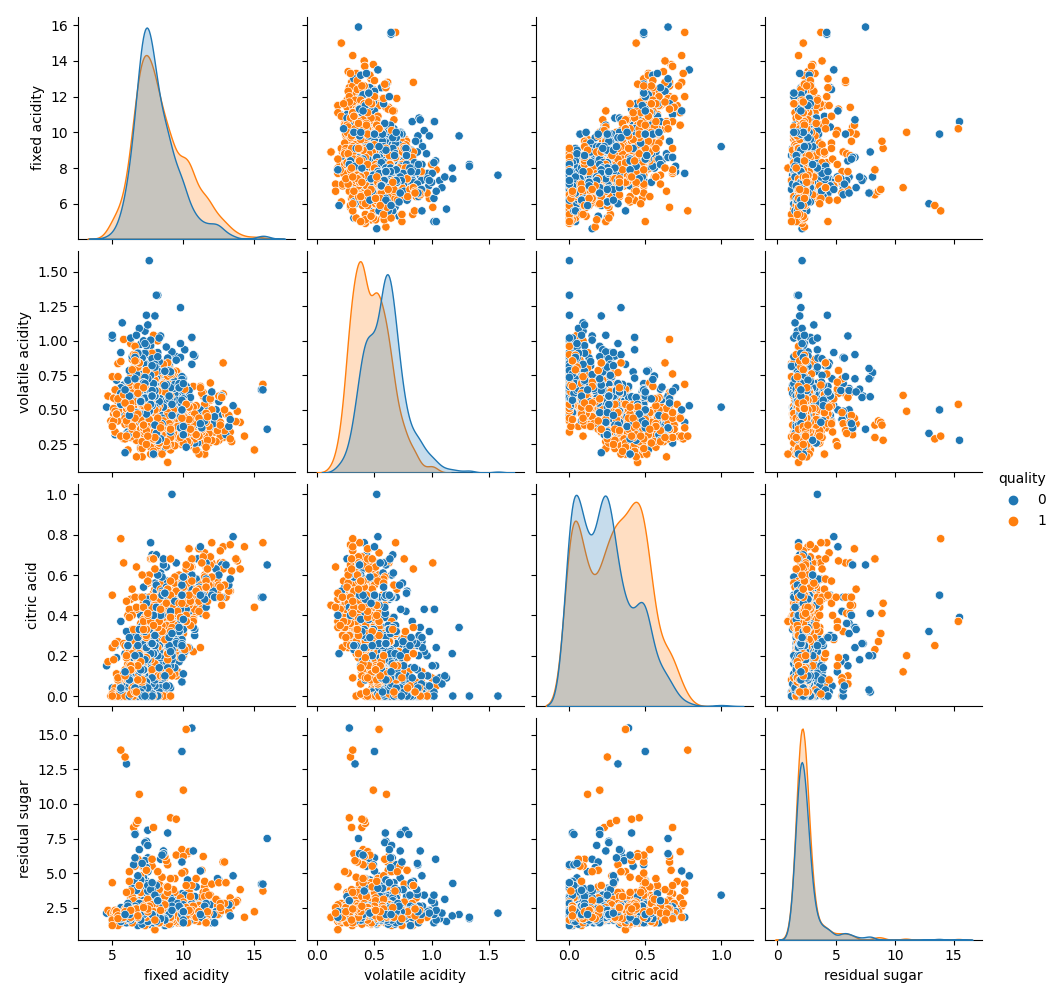
\includegraphics[width=\columnwidth]{../figs/fig-1.png}
	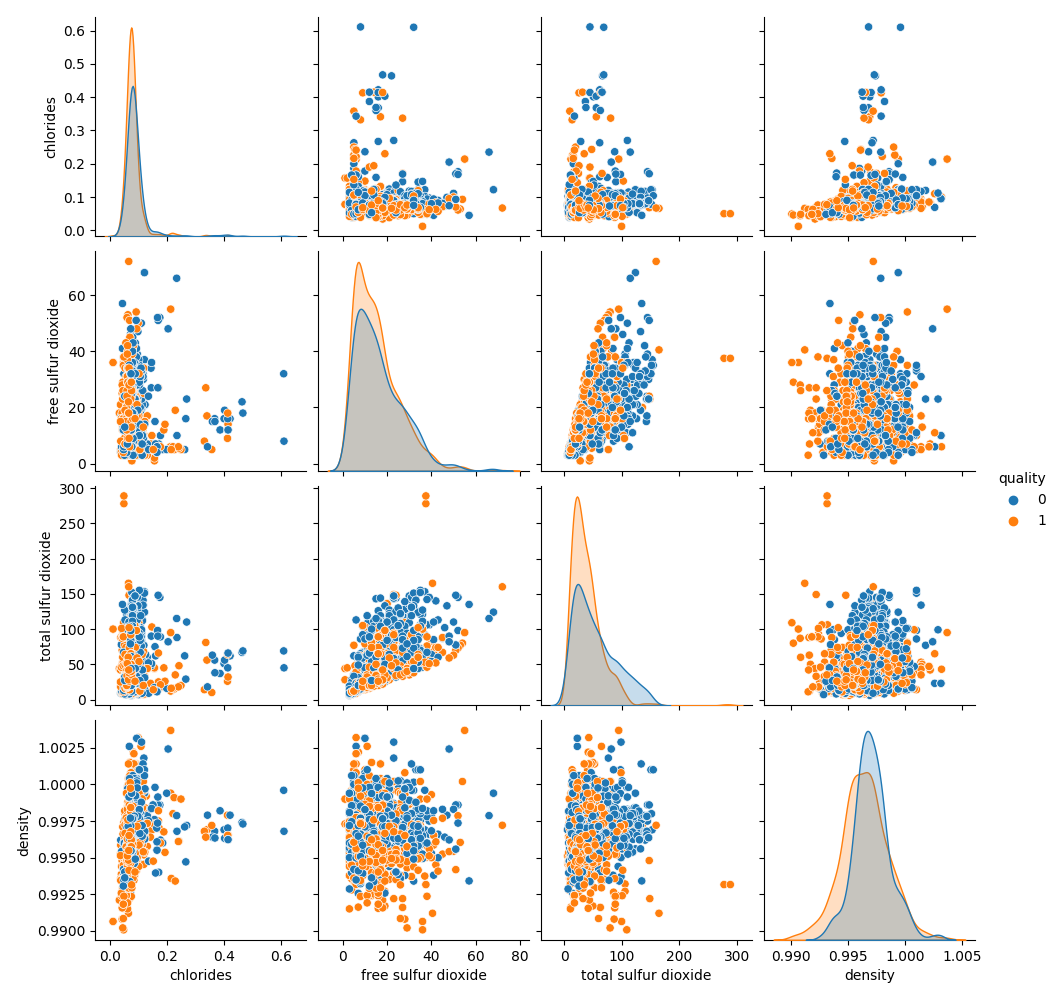
\includegraphics[width=\columnwidth]{../figs/fig-2.png}
	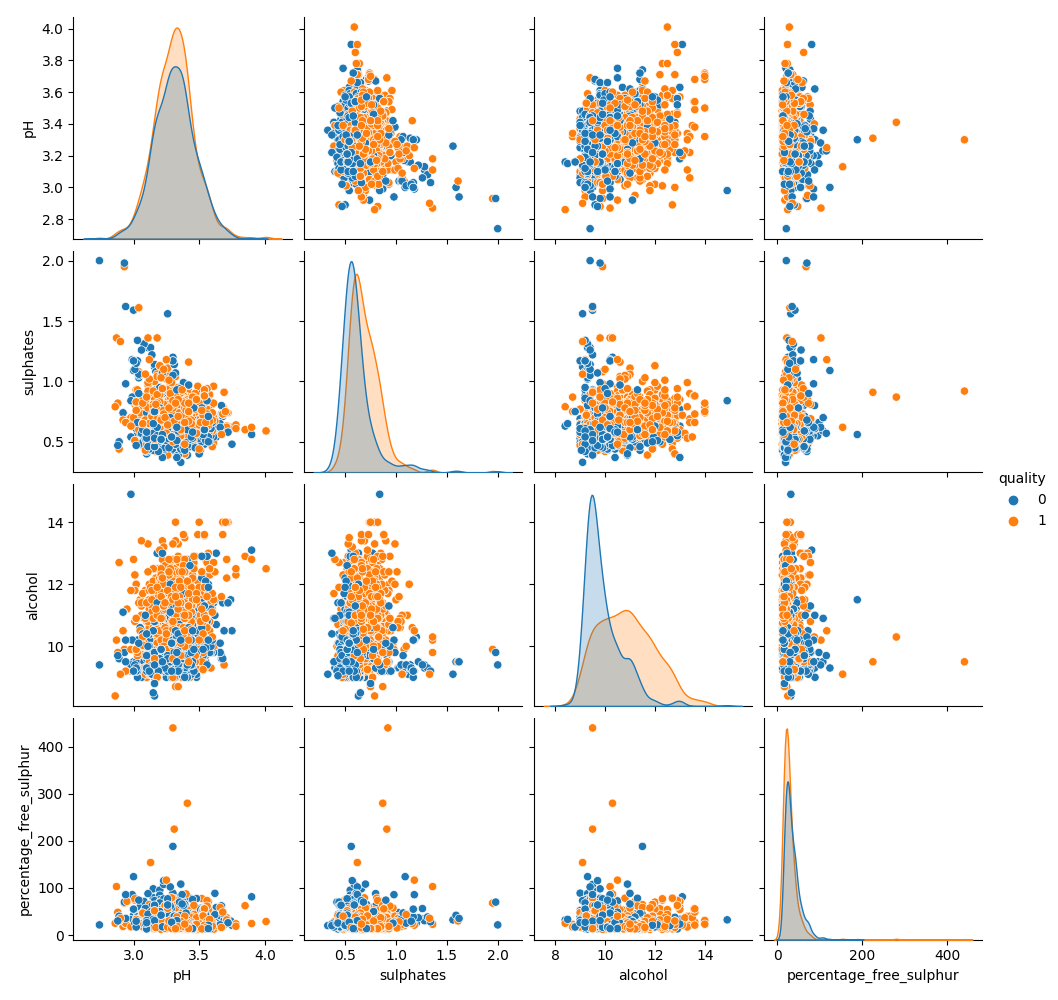
\includegraphics[width=\columnwidth]{../figs/fig-3.png}
	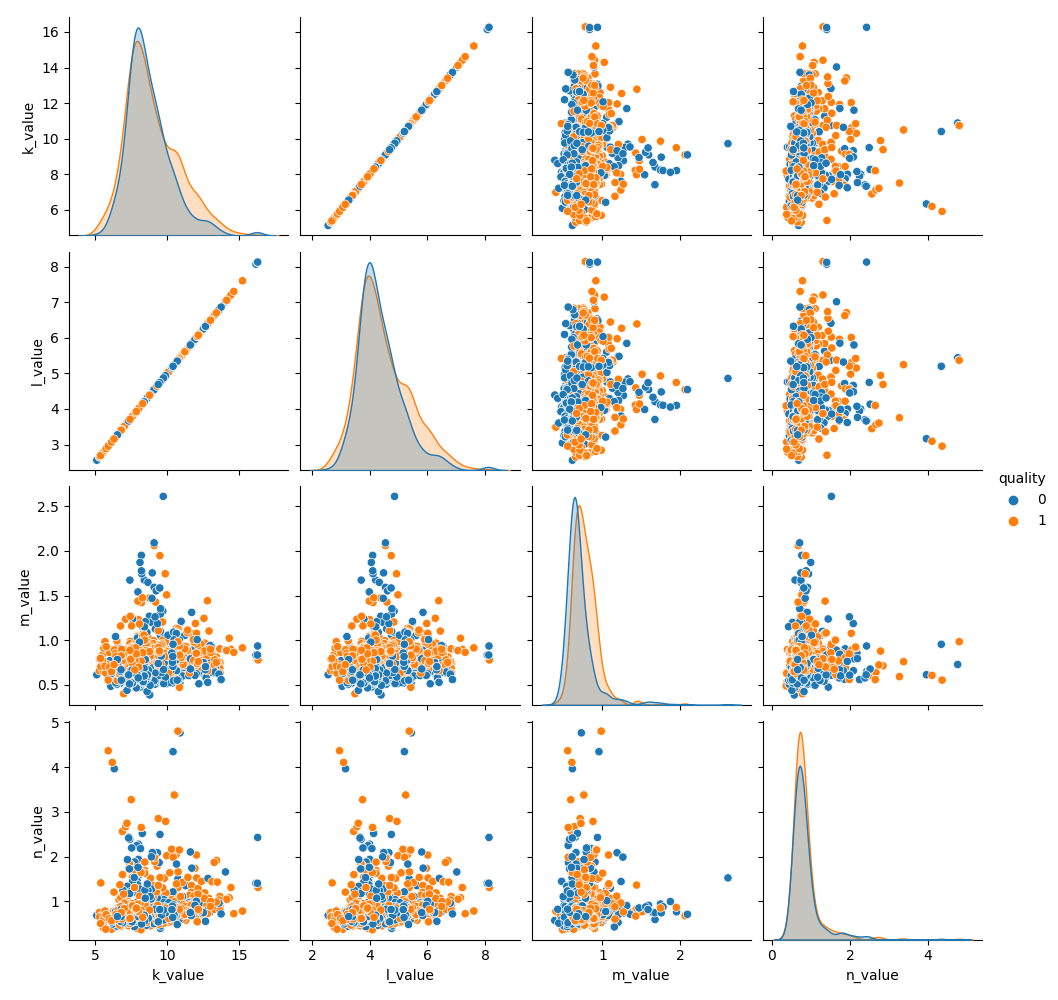
\includegraphics[width=\columnwidth]{../figs/fig-4.png}
	
	Observe that the plot of \pyth{'k_value'} vs \pyth{'l_value'} is a straight line, which suggests that they are linearly dependent on each other.
	\pagebreak
	
	\section{Training the model}
	First, we randomly split our data set into training and test data sets in the ratio $80:20$
	\begin{python}
	training_indices = random.sample(range(total_count), int(0.8 * total_count)) \end{python}
	\pyth{random.sample} chooses a random subset (of indices) of size $= \lfloor 0.8 \times 1598 \rfloor = 1279$ from the set $\{0, 1, 2, \ldots, 1599 \}$. We consider the samples (without the \pyth{'quality'} column) of the data set corresponding to these indices to be our training data set and the rest as our test data set. We store the values of the 'quality' column corresponding to these indices as \pyth{'training_labels'} and \pyth{'test_labels'} respectively.
	
	\subsection*{The Logistic Regression Model}
	We use a logistic regression model for this classification problem.	 
	
	We are given $N = 1599$ labelled samples $\{(\vec{x}_i, y_i)\}, \quad i = 1,2,\ldots,N$
	
	For this problem, we choose the sigmoid function to model our probability.
	\begin{align}
		S(x) &= \frac{1}{1 + e^{-x}} \\
		1 - S(x) &= 1 - \frac{1}{1 + e^{-x}} \\
		&= \frac{1 + e^{-x} - 1}{1 + e^{-x}} \\
		&= \frac{e^{-x}}{1 + e^{-x}} \\
		&= \frac{1}{1 + e^{x}} \\
		&= S(-x)
	\end{align}
	
	Our goal is to find a weight vector $\vec{w}$ that maximizes the log-likelihood
	\begin{align}
		J = \frac{1}{N} \sum_{i=1}^N y_i \log (S(z)) + (1 - y_i) \log (1 - S(z))
	\end{align}
	
	where $z_i = \vec{w} \cdot \vec{x}_i$
	\begin{align}
		J &= \frac{1}{N} \sum_{i=1}^N y_i \log (S(z_i)) + (1 - y_i) \log (1 - S(z_i)) \\
		&= \frac{1}{N} \sum_{i=1}^N y_i \log \brak{\frac{1}{1 + e^{-z_i}}} + (1 - y_i) \log \brak{\frac{1}{1 + e^{z_i}}} \\
		&= -\frac{1}{N} \sum_{i=1}^N y_i \log \brak{1 + e^{-z_i}} + (1 - y_i) \log \brak{1 + e^{z_i}} \\
		\implies -J &=  \frac{1}{N} \sum_{i=1}^N y_i ~ \mathrm{log1p} \brak{e^{-z_i}} + (1 - y_i) ~ \mathrm{log1p} \brak{e^{z_i}} \\
	\end{align}
	
	where $\mathrm{log1p(x)} = \log(1+x)$
	
	Maximizing $J$ is equivalent to minimizing $J$
	
	$\mathrm{log1p(x)}$ is being used, because in Python, \pyth{log1p(x)} is more precise than \pyth{log(1 + x)} when $x \ll 1$
	\pagebreak
	
	\subsection*{Gradient of the log-likelihood function}
	We will now compute the gradient of the negative of the log-likelihood function, which we are going to need later
	
	For the sake of simplicity, let $N = 2$ and $\vec{x}_i$ be two-dimensional vectors \myvec{x_{ia} & x_{ib}}
	\begin{align}
		-J &= \frac{1}{N} \sum_{i=1}^N y_i \log \brak{1 + e^{-z}} + (1 - y_i) \log \brak{1 + e^{z}} \\
		&= \frac{1}{2} \brak{y_1 \log \brak{1 + e^{-z_1}} + (1 - y_1) \log \brak{1 + e^{z_1}} + y_2 \log \brak{1 + e^{-z_2}} + (1 - y_2) \log \brak{1 + e^{z_2}}} 
	\end{align}
	
	Now, let $\vec{w} = \myvec{w_a & w_b}$
	\begin{align}
		\nabla (-J) &= \myvec{\dfrac{\partial (-J)}{\partial w_a} & \dfrac{\partial (-J)}{\partial w_b}} \\
		&= \frac{1}{2} \myvec{y_1  \dfrac{1}{1 + e^{-z_1}} (-e^{-z_1}) \dfrac{\partial z_1}{\partial w_a} + (1 - y_1) \dfrac{1}{1 + e^{z_1}} e^{z_1} \dfrac{\partial z_1}{\partial w_a} + \cdots & \cdots}
	\end{align}
	
	Now, $z_1 = \vec{w} \cdot \vec{x}_1 = w_a x_{1a} + w_b x_{1b}$
	\begin{align}
		\implies \dfrac{\partial z_1}{\partial w_a} = x_{1a}, \qquad \dfrac{\partial z_1}{\partial w_b} = x_{1b} 
	\end{align}
	
	Similarly, 
	\begin{align}
		\implies \dfrac{\partial z_2}{\partial w_a} = x_{2a}, \qquad \dfrac{\partial z_2}{\partial w_b} = x_{2b} 
	\end{align}
	
	\begin{align}
		\nabla (-J) = \frac{1}{2} \myvec{-y_1 S(-z_1) x_{1a} + (1 - y_1) S(z_1) x_{1a} + \cdots & \cdots}
	\end{align}
	
	Now,
	\begin{align}
		-y_1 S(-z_1) x_{1a} + (1 - y_1) S(z_1) x_{1a} &= -y_1 (1 - S(z_1)) x_{1a} + (1 - y_1) S(z_1) x_{1a} \\		
		&= -y_1x_{1a} + y_1x_{1a}S(z_1) + x_{1a}S(z_1) - y_1x_{1a}S(z_1) \\
		&= x_{1a} (S(z_1) - y_1)
	\end{align}
	
	Thus,
	\begin{align}
		\nabla (-J) &= \frac{1}{2} \myvec{x_{1a} (S(z_1) - y_1) + x_{2a} (S(z_2) - y_2) & x_{1b} (S(z_1) - y_1) + x_{2b} (S(z_2) - y_2)} \\
		&= \frac{1}{2} \myvec{x_{1a} & x_{2a} \\ x_{1b} & x_{2b}} \myvec{S(z_1) - y_1 \\ S(z_2) - y_2} \\
		&= \frac{1}{2} \vec{X}^T \myvec{S(z_1) - y_1 \\ S(z_2) - y_2}
	\end{align}
	
	where $\vec{X} = \myvec{x_{1a} & x_{1b} \\ x_{2a} & x_{2b}}$ is the training data set
	
	\vspace*{10pt}
	Therefore, the code for calculating the gradient is given by
	\begin{python}
	def gradient(X, y, W):
    		z = np.dot(X, W)
    		return np.dot(X.T, sigmoid(z) - y) / len(X) \end{python}
	
	\pagebreak
	
	\subsection*{Steepest Descent Algorithm}
	We use the steepest descent algorithm to compute the optimal $\vec{w}$ that minimizes the cost function $C$ \\(in our case $C = -J$) 	
	
	The algorithm is given by:
	\begin{enumerate}
		\item Initialize $\vec{w} = \vec{w}^{(0)}$
		\item Compute the gradient $g^{(k)} = \nabla C(\vec{w}^{(k)})$
		\item At the next iteration, set $\vec{w}^{(k+1)} = \vec{w}^{(k)} - t_k g^{(k)}$ where $t_k$ is the step size (constant in our model)
		\item Keep iterating over $k$ until $\nabla C(\vec{w}^{(k)})$ is sufficiently small 	
	\end{enumerate}
	
	\vspace*{20pt}
	The code for this is:
	\begin{python}
	def steepest_descent(X, y):
    		W = np.zeros(len(X.columns)) # Initial guess
    		epsilon = 1e-6 
    		step_size = 1e-2 
    		g_prev = gradient(X, y, W)
    		W -= step_size * g_prev
    		g_curr = gradient(X, y, W)

    		while (abs(np.linalg.norm(g_curr) - np.linalg.norm(g_prev)) > epsilon): 
        		g_prev = g_curr
        		W -= step_size * g_curr
        		g_curr = gradient(X, y, W)

    		return W \end{python}
    		
    		For a fixed step size, it is possible that $\nabla C(\vec{w}^{(k)})$ will just keep oscillating around the minima. In order to prevent that, we have set the break condition so that if the norm of $\nabla C(\vec{w}^{(k)})$ doesn't change significantly, i.e., is negligibly small, we break out of the loop. 
    		
    		This is because, when $\nabla C(\vec{w}^{(k)})$ oscillates around the minima, $\nabla C(\vec{w}^{(k)})$ doesn't approach zero, but its norm remains roughly the same.
    		
    		\vspace*{30pt}
    		All that's left now is training this model on our training data set and finding the optimal weight vector. We do that by executing the following code:
    		\begin{python}
    		weight_vector = steepest_descent(training_set, training_labels) \end{python}
    		
    		The following are the evaluation metrics obtained after running this model on our test data set:
    		\begin{align}
    			\text{Accuracy } &= 0.603125 \\
    			\text{Precision } &= 0.581081081081081 \\
    			\text{Recall/Sensitivity } &= 0.9828571428571429 \\
    			\text{Specificity } &= 0.14482758620689656 
    		\end{align}
	
\end{document}
